%----------------------------------------------------------------------------------------
%	PACKAGES AND OTHER DOCUMENT CONFIGURATIONS
%----------------------------------------------------------------------------------------

\documentclass[11pt]{diazessay} % Font size (can be 10pt, 11pt or 12pt)
\usepackage{float}
\usepackage{sectsty}
\usepackage[numbers]{natbib}
\sectionfont{\centering}
\usepackage{listings}
\usepackage{color}

\definecolor{dkgreen}{rgb}{0,0.6,0}
\definecolor{gray}{rgb}{0.5,0.5,0.5}
\definecolor{mauve}{rgb}{0.58,0,0.82}

\lstset{frame=tb,
  language=php,
  aboveskip=3mm,
  belowskip=3mm,
  showstringspaces=false,
  columns=flexible,
  basicstyle={\small\ttfamily},
  numbers=none,
  numberstyle=\tiny\color{gray},
  keywordstyle=\color{blue},
  commentstyle=\color{dkgreen},
  stringstyle=\color{mauve},
  breaklines=true,
  breakatwhitespace=true,
  tabsize=3
}
%----------------------------------------------------------------------------------------
%	TITLE SECTION
%----------------------------------------------------------------------------------------

\title{\textbf{Traffic Analysis} \\ {\Large\itshape A write-up}} % Title and subtitle

\author{\textbf{Matthew Doherty} \\ \textit{Rhodes University}} % Author and institution

\date{\today} % Date, use \date{} for no date

%----------------------------------------------------------------------------------------

\begin{document}

\maketitle % Print the title section

%----------------------------------------------------------------------------------------
%	ABSTRACT AND KEYWORDS
%----------------------------------------------------------------------------------------

%\renewcommand{\abstractname}{Summary} % Uncomment to change the name of the abstract to something else

\renewcommand{\thesection}{\arabic{section}}
\renewcommand{\thesubsection}{\arabic{subsection}}
\renewcommand{\thesubsubsection}{\arabic{subsubsection}}
\renewcommand{\thesubsection}{\thesection.\arabic{subsection}}
\renewcommand{\thesubsubsection}{\thesubsection.\arabic{subsubsection}}

\vspace{30pt} % Vertical whitespace between the abstract and first section

%----------------------------------------------------------------------------------------
%	ESSAY BODY
%----------------------------------------------------------------------------------------

% "*" means no numbering -> \section*{Introduction}

\section{Introduction}



%------------------------------------------------

\section{Traffic Overview}

\begin{figure}[H]
        \centering
        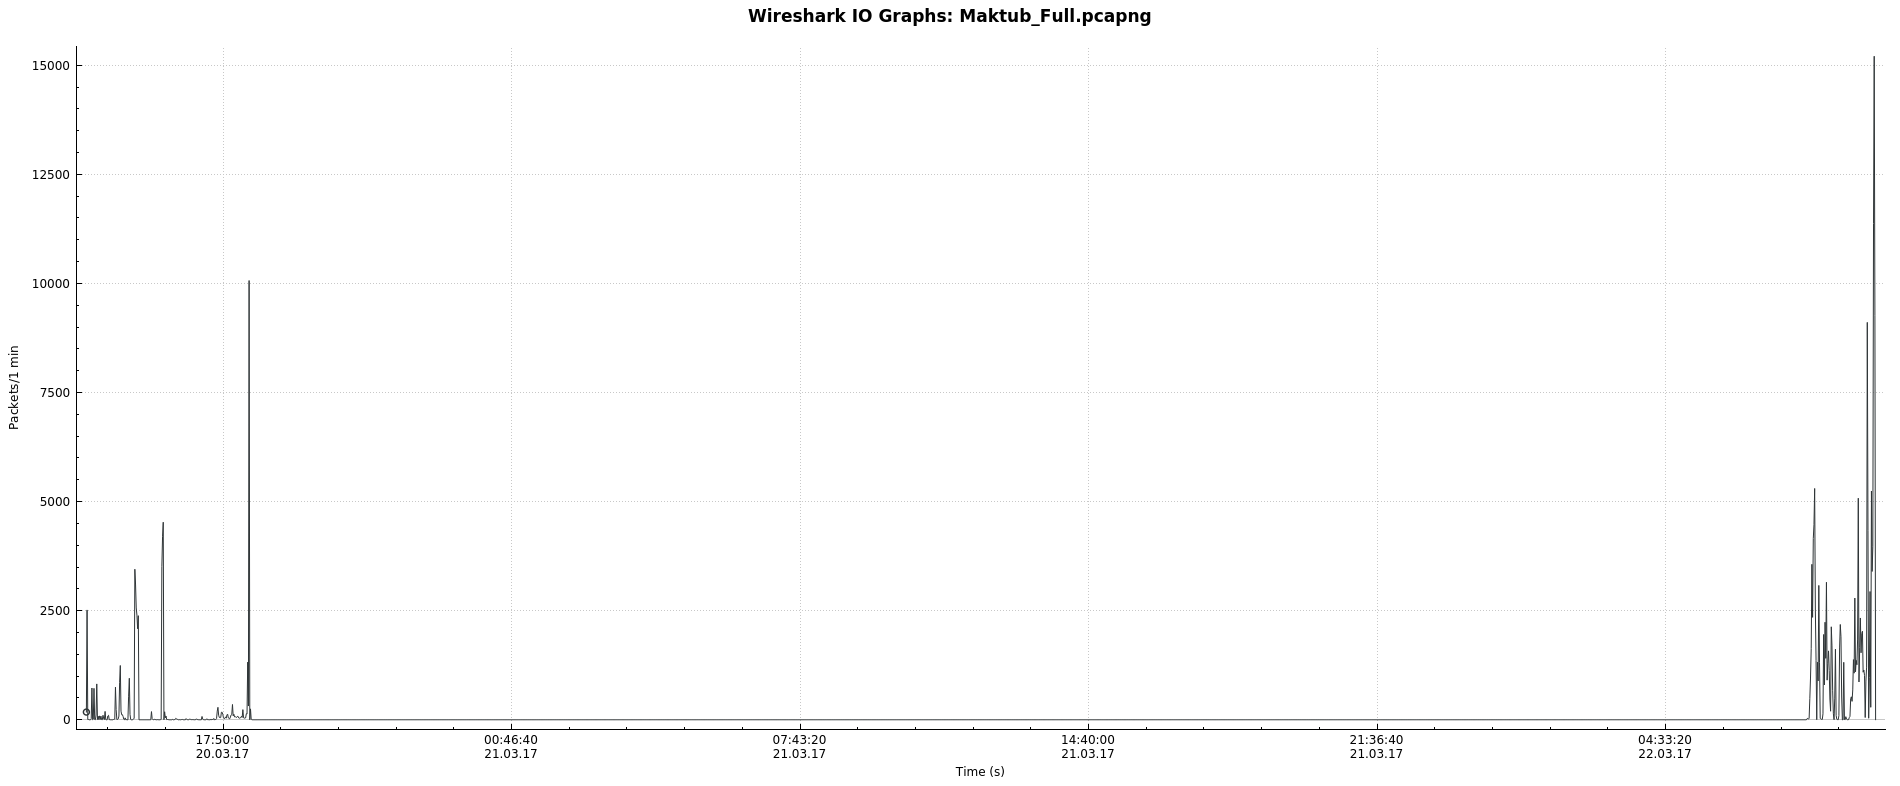
\includegraphics[scale=0.30]{Maktub_Full.png}
    \caption{Pcap Lifetime graph}
\end{figure}

\begin{figure}[H]
        \centering
        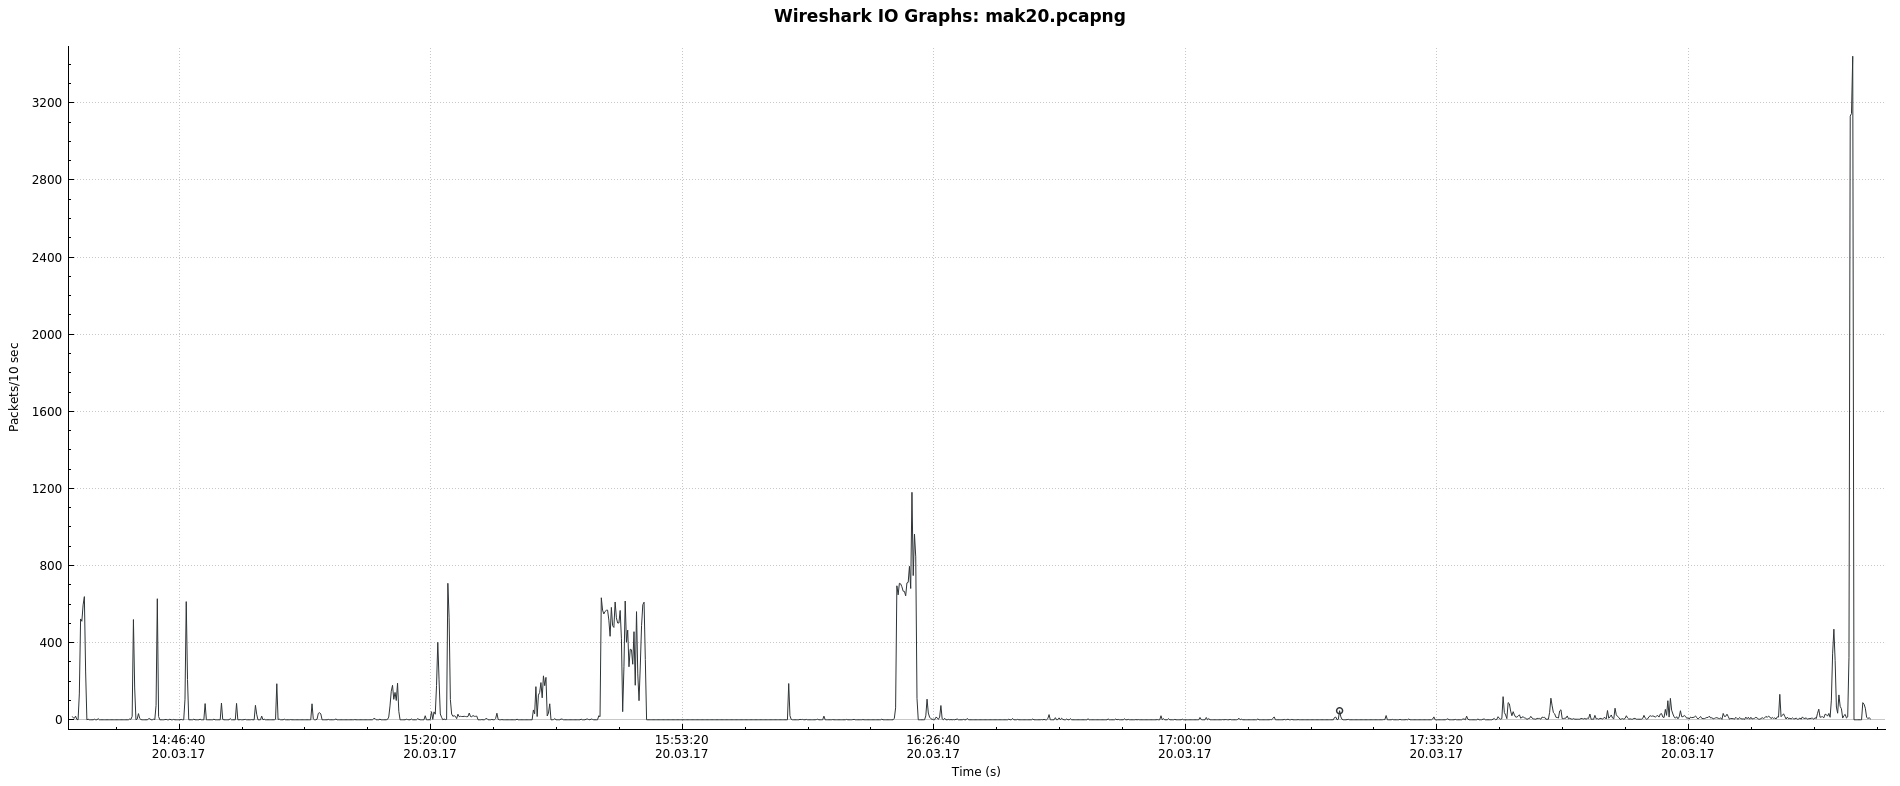
\includegraphics[scale=0.30]{mak20.png}
    \caption{IO graph for 2017-03-20} 
\end{figure}

\begin{figure}[H]
        \centering
        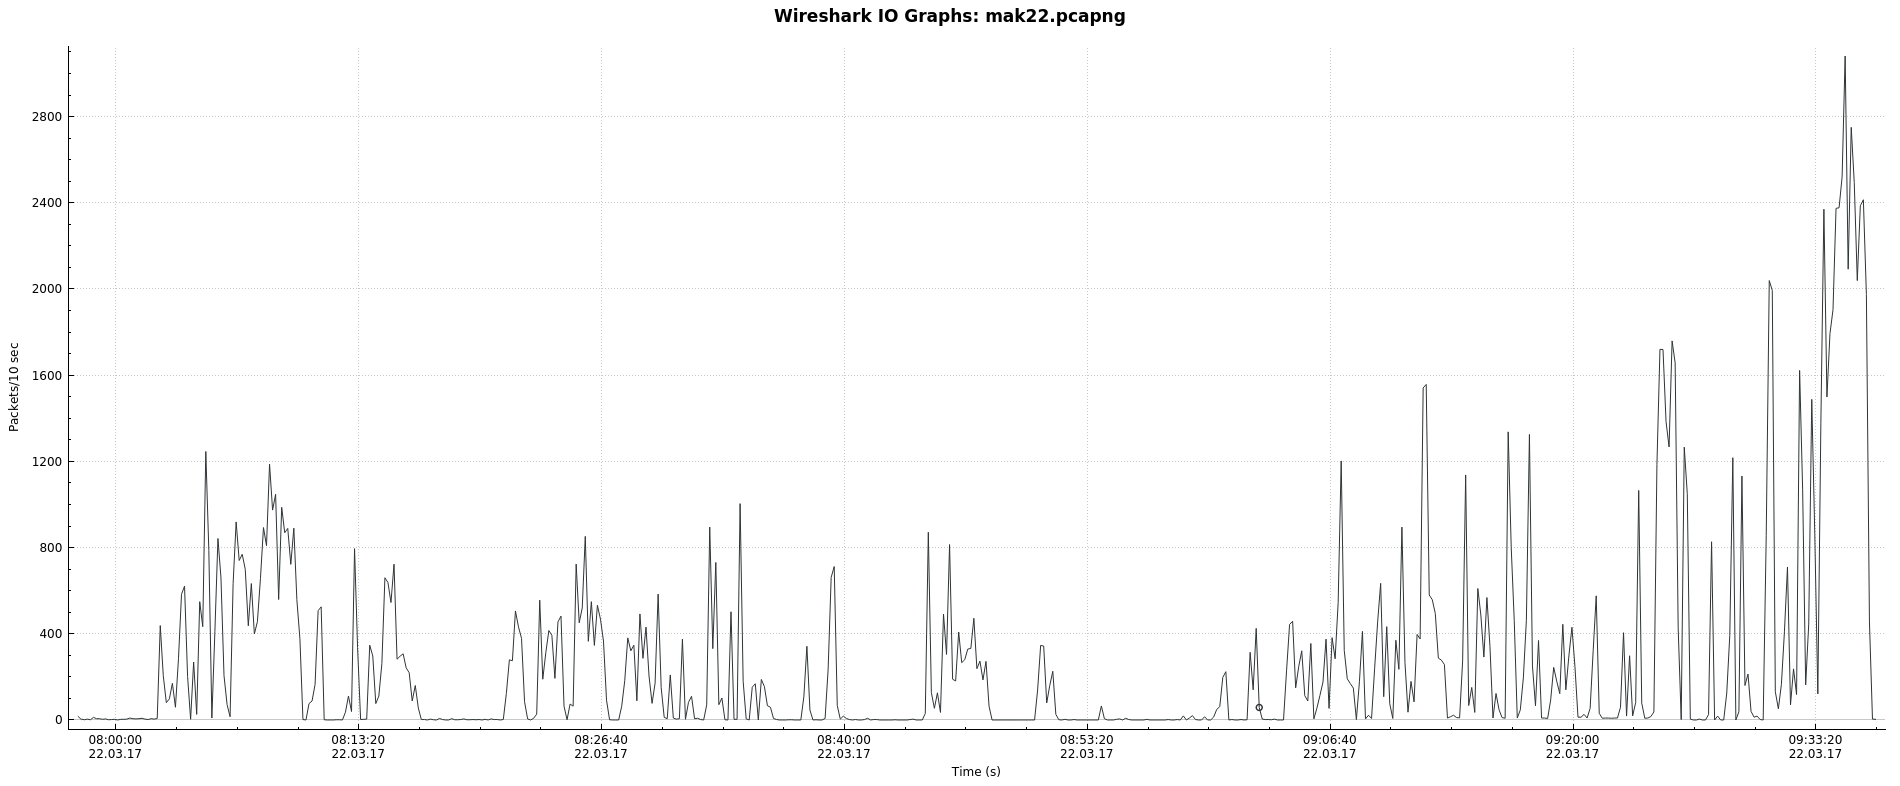
\includegraphics[scale=0.30]{mak22.png}
    \caption{IO Graph for 2017-03-22}
\end{figure}

This analysis examines events that took place on a South African network on the 2017-03-20 and 2017-03-22. We will make the argument, based purely on captured network traffic, that a host was compromised with a ransomware variant known as Maktub. 

The three graphs depict packets per 10 seconds for traffic for a full network capture over the period, followed by traffic generated on the 20th and 22nd. The traffic was divided in this way to logically separate the behavior associated with each time sequence. The story of the infected host is encapsulated on the first day whereas the second day exhibits indirect behavior of the infected host as the machine has been taken offline.  


Legitmate windows update from Ikai CDN 
DNS for onion domain singapoor 
DNS for cryptostorm to establish VPN Germany
Get Windows-CryptoAPI from comodoca 
China DNS req  for 1.83.255.178 

Cryptostorm VPN connect over TLS 
192.36.27.5 -> Amsterdam IP for onion (Entry node)

%------------------------------------------------

\section{Traffic for initial compromise}



%------------------------------------------------

\section{Conclusion}

%----------------------------------------------------------------------------------------
%	BIBLIOGRAPHY
%----------------------------------------------------------------------------------------

\clearpage
%\bibliographystyle{unsrt}
\bibliographystyle{plainnat}
%plainnat, unsrtnat and abbrevnat)
\bibliography{paper.bib}

%----------------------------------------------------------------------------------------

\end{document}
